% Options for packages loaded elsewhere
\PassOptionsToPackage{unicode}{hyperref}
\PassOptionsToPackage{hyphens}{url}
%
\documentclass[
  12pt,
]{article}
\usepackage{lmodern}
\usepackage{amssymb,amsmath}
\usepackage{ifxetex,ifluatex}
\ifnum 0\ifxetex 1\fi\ifluatex 1\fi=0 % if pdftex
  \usepackage[T1]{fontenc}
  \usepackage[utf8]{inputenc}
  \usepackage{textcomp} % provide euro and other symbols
\else % if luatex or xetex
  \usepackage{unicode-math}
  \defaultfontfeatures{Scale=MatchLowercase}
  \defaultfontfeatures[\rmfamily]{Ligatures=TeX,Scale=1}
  \setmainfont[]{Times New Roman}
\fi
% Use upquote if available, for straight quotes in verbatim environments
\IfFileExists{upquote.sty}{\usepackage{upquote}}{}
\IfFileExists{microtype.sty}{% use microtype if available
  \usepackage[]{microtype}
  \UseMicrotypeSet[protrusion]{basicmath} % disable protrusion for tt fonts
}{}
\makeatletter
\@ifundefined{KOMAClassName}{% if non-KOMA class
  \IfFileExists{parskip.sty}{%
    \usepackage{parskip}
  }{% else
    \setlength{\parindent}{0pt}
    \setlength{\parskip}{6pt plus 2pt minus 1pt}}
}{% if KOMA class
  \KOMAoptions{parskip=half}}
\makeatother
\usepackage{xcolor}
\IfFileExists{xurl.sty}{\usepackage{xurl}}{} % add URL line breaks if available
\IfFileExists{bookmark.sty}{\usepackage{bookmark}}{\usepackage{hyperref}}
\hypersetup{
  pdftitle={Visually Representing State and Local Water Shutoff Moratoria During the COVID-19 Pandemic},
  pdfauthor={Simon Warren},
  hidelinks,
  pdfcreator={LaTeX via pandoc}}
\urlstyle{same} % disable monospaced font for URLs
\usepackage[margin=2.54cm]{geometry}
\usepackage{longtable,booktabs}
% Correct order of tables after \paragraph or \subparagraph
\usepackage{etoolbox}
\makeatletter
\patchcmd\longtable{\par}{\if@noskipsec\mbox{}\fi\par}{}{}
\makeatother
% Allow footnotes in longtable head/foot
\IfFileExists{footnotehyper.sty}{\usepackage{footnotehyper}}{\usepackage{footnote}}
\makesavenoteenv{longtable}
\usepackage{graphicx,grffile}
\makeatletter
\def\maxwidth{\ifdim\Gin@nat@width>\linewidth\linewidth\else\Gin@nat@width\fi}
\def\maxheight{\ifdim\Gin@nat@height>\textheight\textheight\else\Gin@nat@height\fi}
\makeatother
% Scale images if necessary, so that they will not overflow the page
% margins by default, and it is still possible to overwrite the defaults
% using explicit options in \includegraphics[width, height, ...]{}
\setkeys{Gin}{width=\maxwidth,height=\maxheight,keepaspectratio}
% Set default figure placement to htbp
\makeatletter
\def\fps@figure{htbp}
\makeatother
\setlength{\emergencystretch}{3em} % prevent overfull lines
\providecommand{\tightlist}{%
  \setlength{\itemsep}{0pt}\setlength{\parskip}{0pt}}
\setcounter{secnumdepth}{5}

\title{Visually Representing State and Local Water Shutoff Moratoria During the
COVID-19 Pandemic}
\usepackage{etoolbox}
\makeatletter
\providecommand{\subtitle}[1]{% add subtitle to \maketitle
  \apptocmd{\@title}{\par {\large #1 \par}}{}{}
}
\makeatother
\subtitle{\url{https://github.com/sbw11/SWarren_Enviro_Data_Proj}}
\author{Simon Warren}
\date{}

\begin{document}
\maketitle

\newpage
\tableofcontents 
\newpage
\listoffigures
\newpage

\hypertarget{rationale-and-research-questions}{%
\section{Rationale and Research
Questions}\label{rationale-and-research-questions}}

Drinking water systems in the United States rely on residential
customers paying their water bills on time in order to fund maintenance,
operations, and infrastructure improvements. To make sure that as many
customers are paying, most systems will disconnect water to residences
or businesses if water bills are overdue by a certain number of days,
and charge a fee to have the water turned back on. The practice has many
names, but one of the most common is ``water shutoffs.'' Activist groups
point out that even in normal circumstances, the practice denies
residents their basic human rights, and that utilities often are biased
in how they use shutoffs-- turning off water to residents who cannot
afford to pay while not continuing water service to large businesses
that are also past-due, but have significant economic influence.
Utilities counter that the measure is necessary to ensure that people do
pay their bills on time.

The COVID-19 pandemic has introduced significant new challenges to water
systems, as the sector tries to support public health and the economy.
U.S. federal guidelines suggest that people wash their hands regularly
and for twenty seconds each time. If a resident's water is shut off,
handwashing is impossible. To make matters worse, the economic shutdown
brought by COVID-19 has hit low-income residents particularly hard, and
made it more challenging for many to pay their bills. As a result, many
states, counties, indigenous areas, cities, towns, and water authorities
have temporarily banned shutoffs, placing moratoria on water shutoffs,
meaning that no one can have their water disconnected. Not all
authorities have required that homes whose water had been shutoff be
reconnected, but some have. It is also worth noting that some states and
municipalities, especially in the North, suspend shutoffs in the
wintertime, and have extended that suspension in light of the pandemic.

The non-profit Food and Water Watch (FWW) has kept a running list of
which authorities have ordered shutoff moratoria, and has used the
information there to advocate for a nation-wide water shutoff ban. The
list updates automatically every 5 minutes, and in mid-March, FWW
published a static map of shutoffs. Based on the list, the Guardian
estimates that 40\% of Americans are living in somewhere that has not
banned shutoffs. Creating a ``live'' map could make this information
more transparent and allow journalists, residents and advocates see
which states and cities have taken the step to ban shutoffs and which
have not, and to see where reconnnections have been ordered.

This report will try to answer four questions:

\begin{enumerate}
\def\labelenumi{\arabic{enumi}.}
\tightlist
\item
  How can FWW's list be turned into a ``live'' map as a tool for
  journalists and residents?
\item
  Is there some spatial relationship between what states and cities are
  ordering moratoria on water shutoffs?
\item
  Is there a spatial relationship between which cities and states are
  instituting reconnections?
\item
  Is there a connection between service population and whether the
  orders include reconnections?
\end{enumerate}

\newpage

\hypertarget{dataset-information}{%
\section{Dataset Information}\label{dataset-information}}

The dataset for this analysis consisted of three pieces: Food and Water
Watch's list, Census TIGER Lines shapefiles to accurately map entities
referenced on the list-- including states, municipalities, and water
authorities-- and a csv file from the U.S. EPA's Safe Drinking Water
Information System (SDWIS), which lists all water districts/authorities.
Water districts do not always have the same political boundaries as the
towns or counties they serve, and the Census does not create a list of
them. SDWIS's list was used to convert terms like ``Anytown Water
Authority'' into a geographical point that would appear in the Census'
shapefiles by matching the authority's name to a county served.

The FWW list was obtained by webscraping the page and converting the
information there into a dataframe, which can update each time the
program is run. This document has information for the type of moratorium
(whether the ban was a moratorium, an extension of a pre-existing one,
or if the authority does not do shutoffs in the first place), the state,
the city/county/authority, the service population covered by the
moratorium, whether restorations are included in the order, and a source
for the order. All but the source were kept. The list was then separated
into three lists-- one of state-level orders, one of orders below the
state level, and one of recognized tribes which do not list a state. In
order to match Census designations and avoid accidentally matching data
to cities with the same name in different states, certain patterns were
inserted into the lists, such as turning all cities/counties into
``Anytown XY'' or ``Any County XY'', capitalizing all water authority
names, and removing ``City'' from New York City, which is listed in the
Census as ``New York.'' SDWIS data was pared down to include only the
name of the water system, the state, and the name of one city, county,
and ZIP code served.

These lists then needed to be attached to shapefiles in order to
visually display which places were instituting moratoria. Since there
are several levels of government issuing the bans, several different
maps were needed in the same place, and so Census TIGER lines were used.
TIGER line files for states, American Indian / Alaska Native / Native
Hawaiian Areas, metropolitan divisions, core-based statistical areas,
urban areas, and counties were imported using the tigris package.
Census-designated places were not used because the file was simply too
large, and if the map were published online, it would take too long to
load.

Below is a list of variables created for the map.

\begin{longtable}[]{@{}lll@{}}
\toprule
\begin{minipage}[b]{0.24\columnwidth}\raggedright
Variables\strut
\end{minipage} & \begin{minipage}[b]{0.58\columnwidth}\raggedright
Units\strut
\end{minipage} & \begin{minipage}[b]{0.09\columnwidth}\raggedright
Source\strut
\end{minipage}\tabularnewline
\midrule
\endhead
\begin{minipage}[t]{0.24\columnwidth}\raggedright
Moratorium Type\strut
\end{minipage} & \begin{minipage}[t]{0.58\columnwidth}\raggedright
Text\strut
\end{minipage} & \begin{minipage}[t]{0.09\columnwidth}\raggedright
FWW\strut
\end{minipage}\tabularnewline
\begin{minipage}[t]{0.24\columnwidth}\raggedright
State\strut
\end{minipage} & \begin{minipage}[t]{0.58\columnwidth}\raggedright
Text-State\strut
\end{minipage} & \begin{minipage}[t]{0.09\columnwidth}\raggedright
FWW\strut
\end{minipage}\tabularnewline
\begin{minipage}[t]{0.24\columnwidth}\raggedright
``City''\strut
\end{minipage} & \begin{minipage}[t]{0.58\columnwidth}\raggedright
Text- Any body issuing a moratorium\strut
\end{minipage} & \begin{minipage}[t]{0.09\columnwidth}\raggedright
FWW\strut
\end{minipage}\tabularnewline
\begin{minipage}[t]{0.24\columnwidth}\raggedright
Service Population\strut
\end{minipage} & \begin{minipage}[t]{0.58\columnwidth}\raggedright
Numeric-Population\strut
\end{minipage} & \begin{minipage}[t]{0.09\columnwidth}\raggedright
FWW\strut
\end{minipage}\tabularnewline
\begin{minipage}[t]{0.24\columnwidth}\raggedright
Counties Served\strut
\end{minipage} & \begin{minipage}[t]{0.58\columnwidth}\raggedright
Text- Translates from Water District to County\strut
\end{minipage} & \begin{minipage}[t]{0.09\columnwidth}\raggedright
SDWIS\strut
\end{minipage}\tabularnewline
\begin{minipage}[t]{0.24\columnwidth}\raggedright
State\strut
\end{minipage} & \begin{minipage}[t]{0.58\columnwidth}\raggedright
Polygon-``States''\strut
\end{minipage} & \begin{minipage}[t]{0.09\columnwidth}\raggedright
TIGER Lines\strut
\end{minipage}\tabularnewline
\begin{minipage}[t]{0.24\columnwidth}\raggedright
County\strut
\end{minipage} & \begin{minipage}[t]{0.58\columnwidth}\raggedright
Polygon-``Counties''\strut
\end{minipage} & \begin{minipage}[t]{0.09\columnwidth}\raggedright
TIGER Lines\strut
\end{minipage}\tabularnewline
\begin{minipage}[t]{0.24\columnwidth}\raggedright
Native Area\strut
\end{minipage} & \begin{minipage}[t]{0.58\columnwidth}\raggedright
Polygon-" American Indian / Alaska Native / Native Hawaiian Areas"\strut
\end{minipage} & \begin{minipage}[t]{0.09\columnwidth}\raggedright
TIGER Lines\strut
\end{minipage}\tabularnewline
\begin{minipage}[t]{0.24\columnwidth}\raggedright
Metropolises (2.5 million+)\strut
\end{minipage} & \begin{minipage}[t]{0.58\columnwidth}\raggedright
Polygon-``Metropolitan Divisions''\strut
\end{minipage} & \begin{minipage}[t]{0.09\columnwidth}\raggedright
TIGER Lines\strut
\end{minipage}\tabularnewline
\begin{minipage}[t]{0.24\columnwidth}\raggedright
Cities\strut
\end{minipage} & \begin{minipage}[t]{0.58\columnwidth}\raggedright
Polygon-``Urban Areas''\strut
\end{minipage} & \begin{minipage}[t]{0.09\columnwidth}\raggedright
TIGER Lines\strut
\end{minipage}\tabularnewline
\begin{minipage}[t]{0.24\columnwidth}\raggedright
Towns\strut
\end{minipage} & \begin{minipage}[t]{0.58\columnwidth}\raggedright
Polygon-``Core-Based Statistical Areas''\strut
\end{minipage} & \begin{minipage}[t]{0.09\columnwidth}\raggedright
TIGER Lines\strut
\end{minipage}\tabularnewline
\bottomrule
\end{longtable}

\newpage

\hypertarget{exploratory-analysis}{%
\section{Exploratory Analysis}\label{exploratory-analysis}}

The shapefiles were then joined with their respective moratoria lists,
matching place names where appropriate, and any polygons that were
unmatched to a specific entry in the FWW list were dropped, leaving only
polygons which show the geographic extent of as many moratoria as
possible.

The resulting map shows how much landmass of the country is covered by
these moratoria, but does not identify the size of any given population.
As different layers were created, their tabular data was saved as an
additional dataframe to more easily check for errors.

An initial look shows that several states, cities, counties, tribes, and
towns are ordering a stop to water shutoffs, most are not mandating
restoration of services, and large states like New York, Florida, Texas
have not ordered state-wide moratoria. \newpage

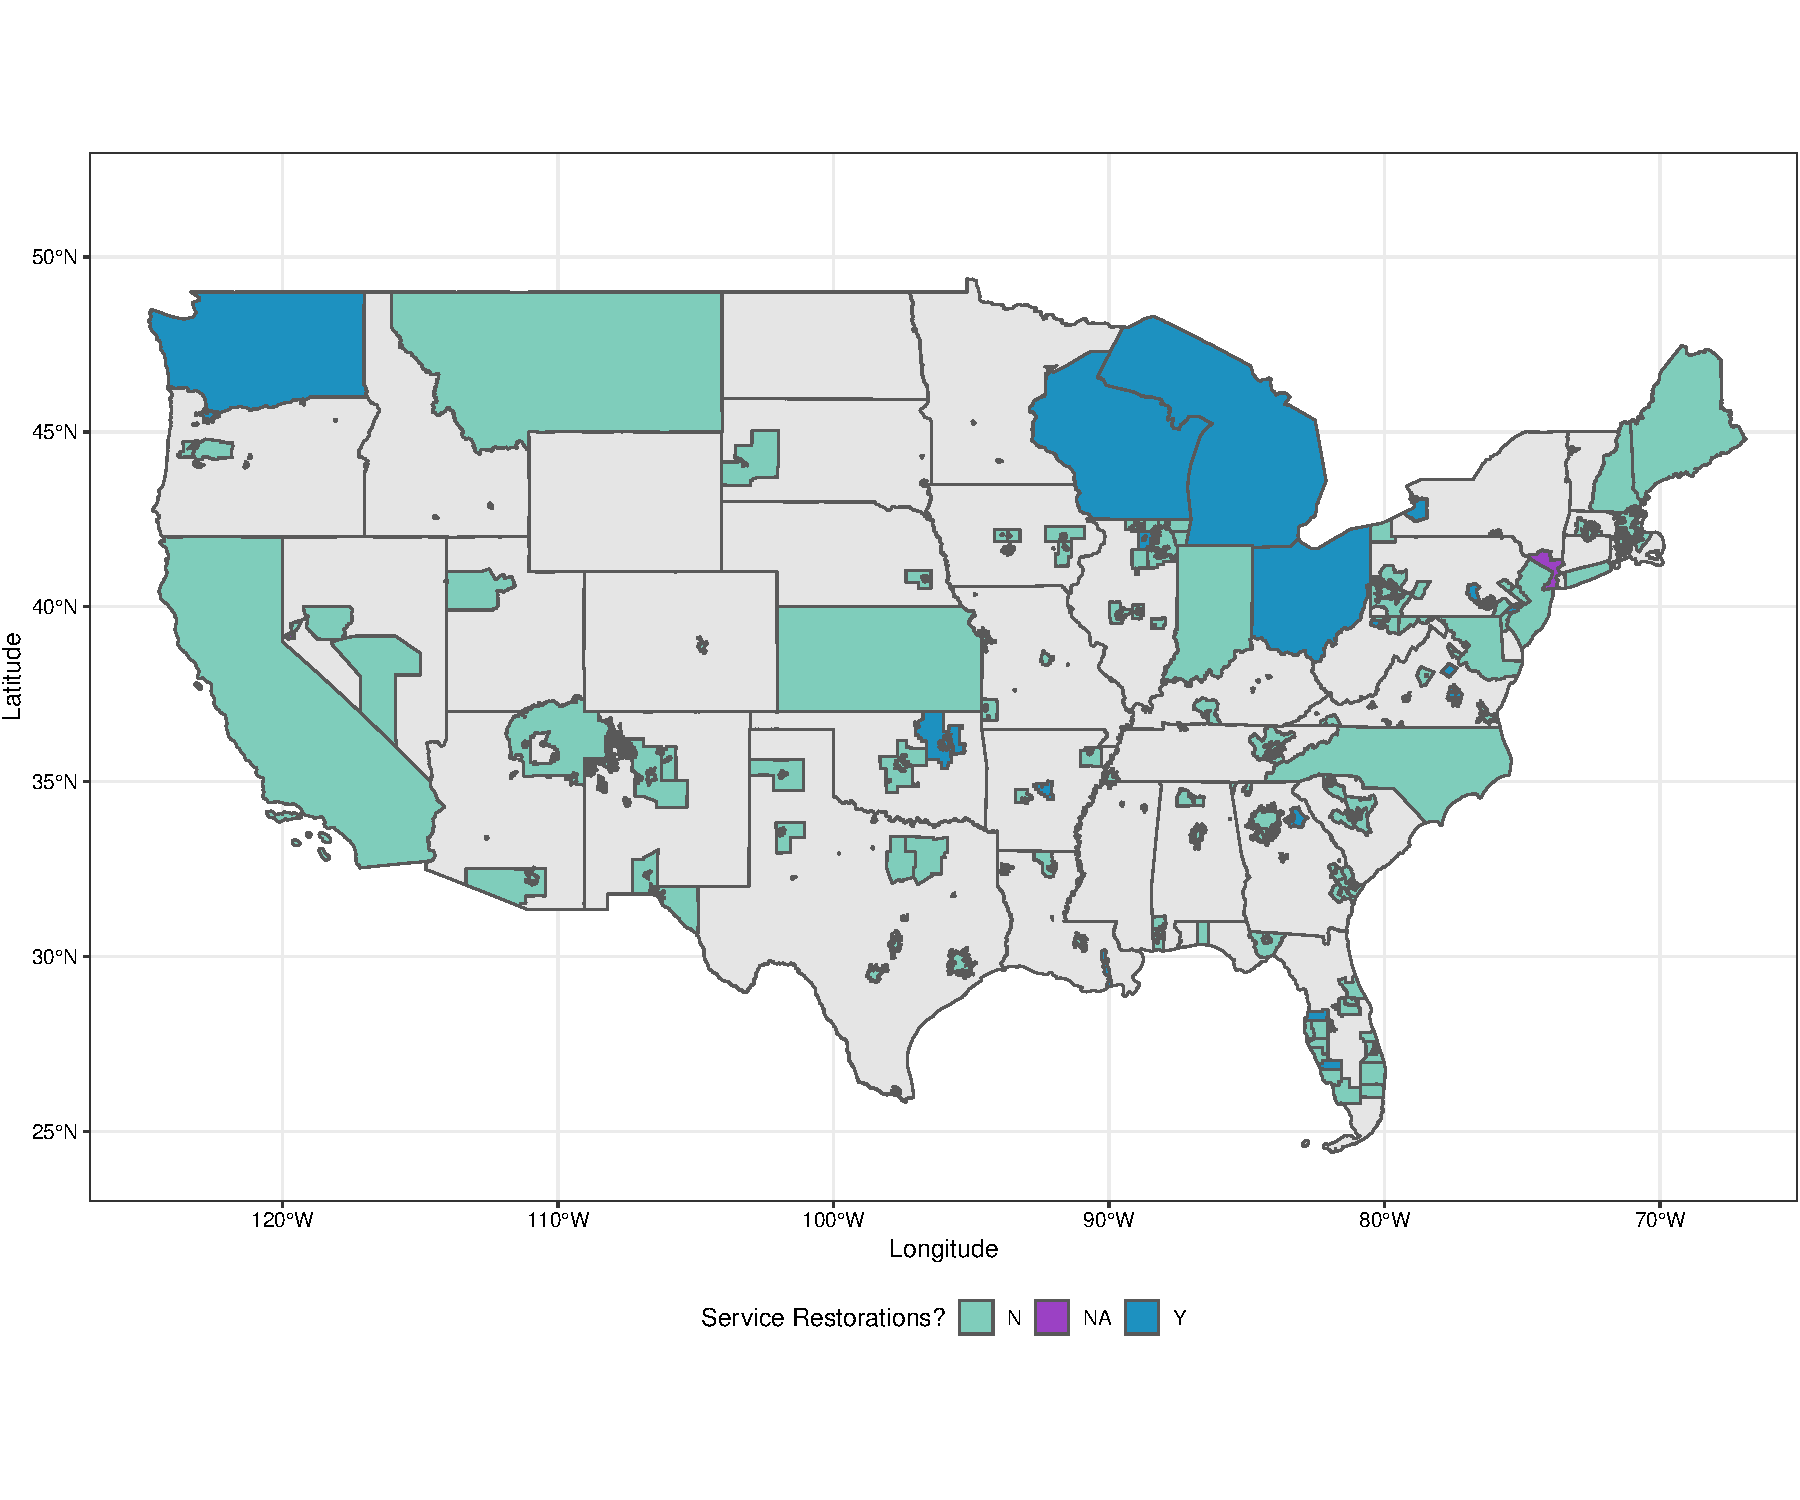
\includegraphics{Warren_ENV872_Project_files/figure-latex/unnamed-chunk-3-1.pdf}

\begin{figure}
\centering
\includegraphics{Warren_ENV872_Project_files/figure-latex/unnamed-chunk-5-1.pdf}
\caption{States and Cities with Water Shutoff Moratoria Under COVID-19}
\end{figure}

\newpage

\hypertarget{analysis}{%
\section{Analysis}\label{analysis}}

FWW's list can be turned into an automatically updating map, although
with some limitations. When looking at both the maps of populations and
coverage, we see some spatial patterns, although these were not
statistically investigated.

\hypertarget{how-can-fwws-list-be-turned-into-a-live-map-as-a-tool-for-journalists-and-residents}{%
\subsection{How can FWW's list be turned into a ``live'' map as a tool
for journalists and
residents?}\label{how-can-fwws-list-be-turned-into-a-live-map-as-a-tool-for-journalists-and-residents}}

This service population map can be turned into a web app using Shiny,
and can be updated automatically. For an automatically-updating map to
continue working and to accurately incorporate all possible
municipalities, extra lines of code need to be written using the
Census-designated places. Similarly, the map will need to be hosted on a
website or server that can download all of the necessary shapefiles,
since a broken internet connection can prevent the shapefiles from
loaded if run each time.

While the initial coverage map shows the geographic extent of shutoff
moratoria, it does little to show how many people are covered by the
orders, and using a color aesthetic to show service populations would
cause California's large population to drown out most other service
populations. As a result, centroids were created for every polygon, so
that each authority is represented as a single point, and all points
were combined into a single map. Then, the size of the points was set to
represent the relative size of the populations covered by the orders.
The result can be seen on the next page.

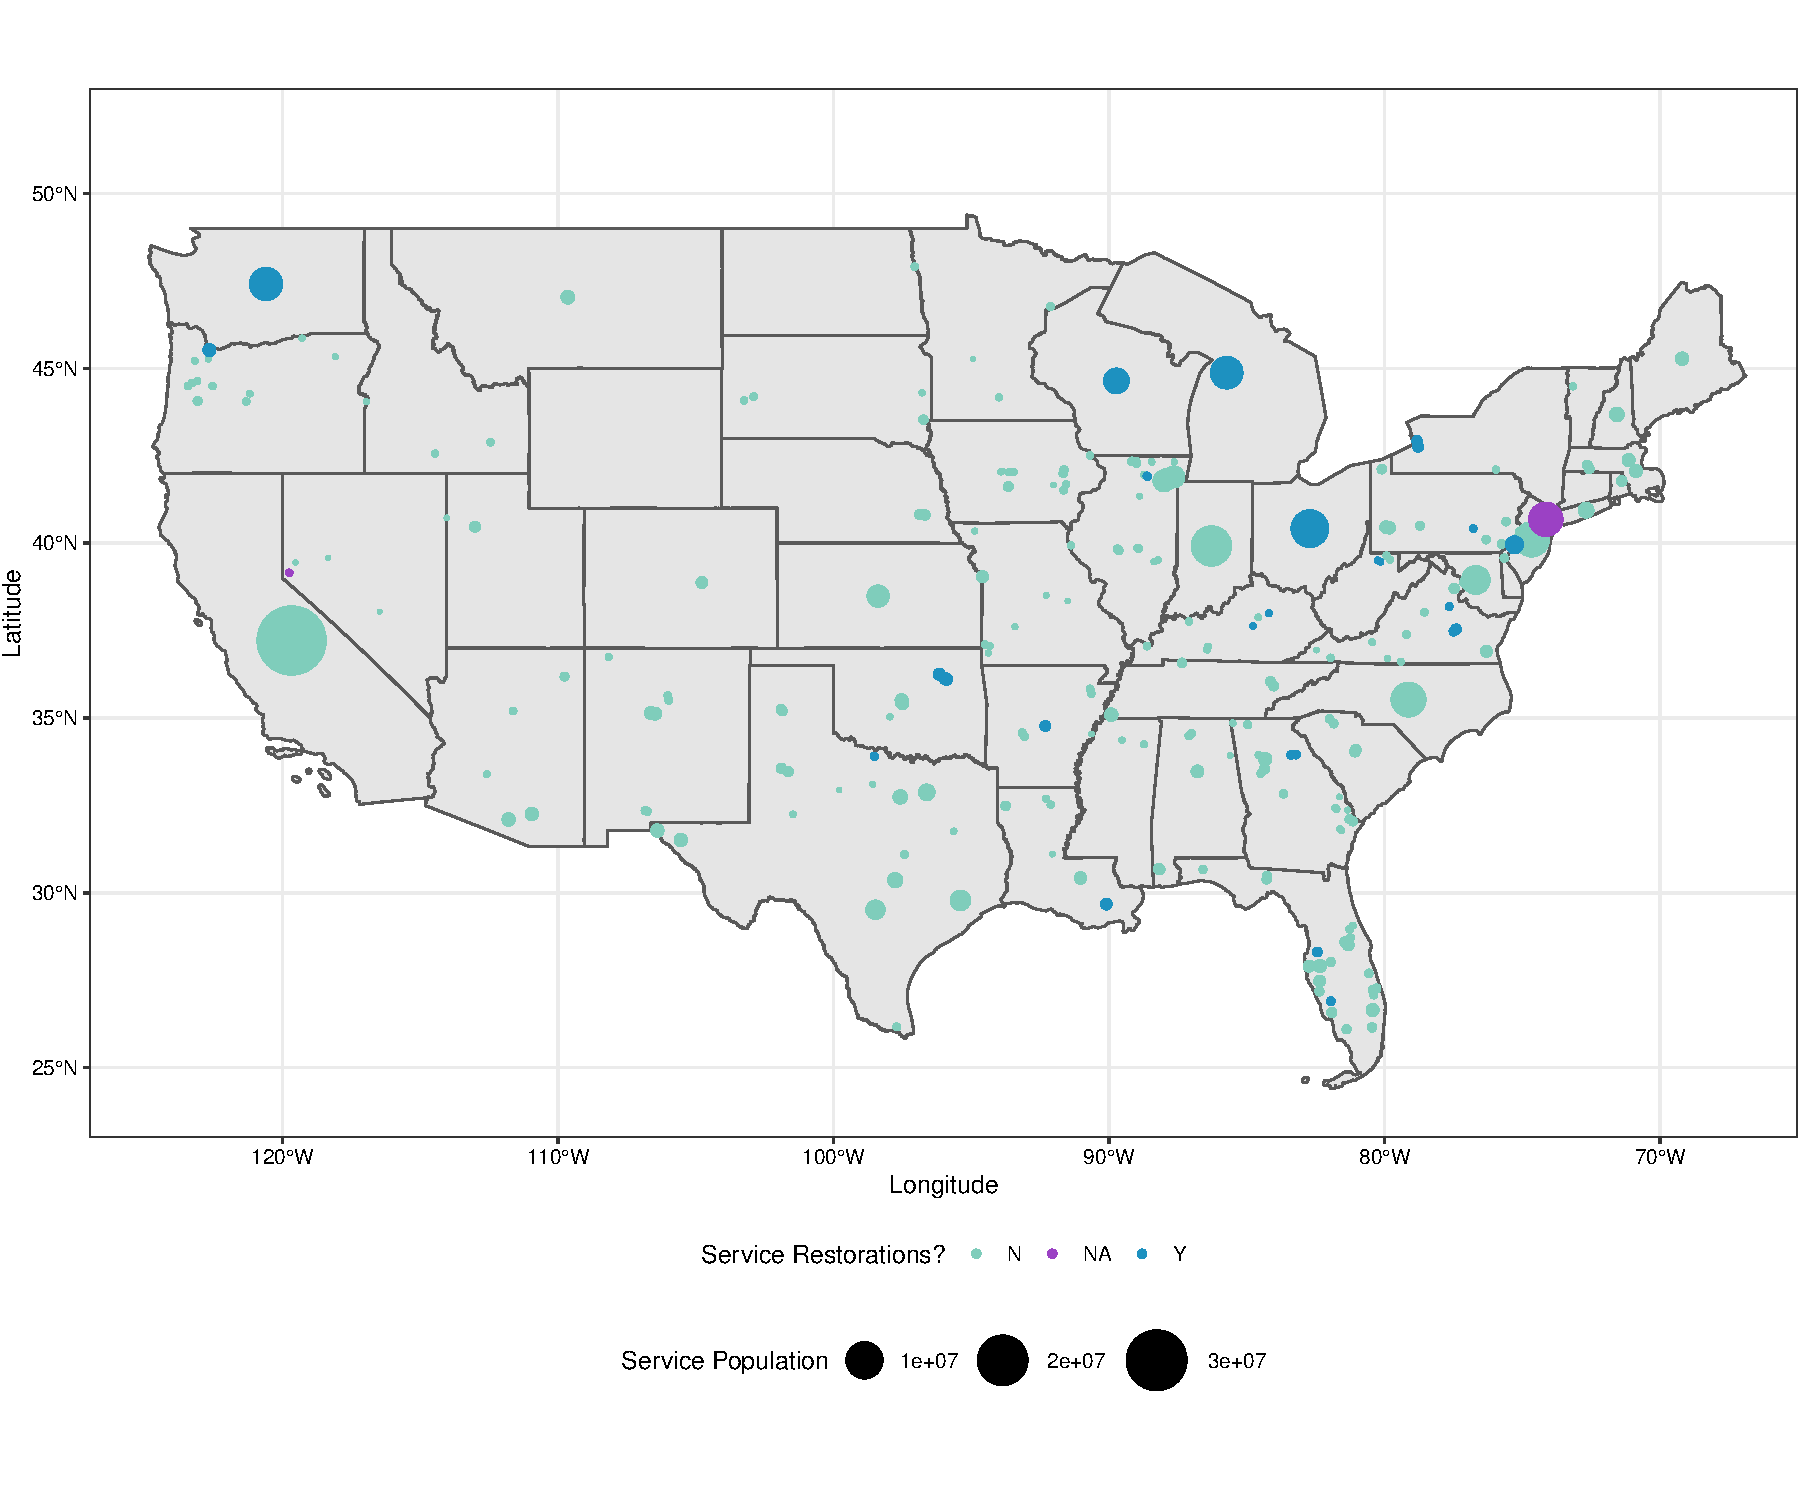
\includegraphics{Warren_ENV872_Project_files/figure-latex/unnamed-chunk-6-1.pdf}

\begin{figure}
\centering
\includegraphics{Warren_ENV872_Project_files/figure-latex/unnamed-chunk-7-1.pdf}
\caption{Population Covered by Water Shutoff Moratoria Under COVID-19}
\end{figure}

\newpage

\hypertarget{is-there-some-spatial-relationship-between-what-states-and-cities-are-ordering-moratoria-on-water-shutoffs}{%
\subsection{Is there some spatial relationship between what states and
cities are ordering moratoria on water
shutoffs?}\label{is-there-some-spatial-relationship-between-what-states-and-cities-are-ordering-moratoria-on-water-shutoffs}}

The initial coverage map indicates that there is at least a qualitative
relationship between location and water shutoffs at the state level, one
which appears to influence cities in nearby states as well. Neighboring
Midwestern states like Ohio, Indiana, Wisconsin, and Michigan have
passed shutoff moratoria, and Ohio, Wisconsin, and Michigan have gone a
step furhter and ordered reconnections as well. This may be because
these states have a history of suspending shutoffs in the wintertime,
and because water justice issues are especially politically sensitive in
Michigan. While Illinois has not issued a statewide order as of April
24, 2020, Chicago has, as have several other communities in the region.

The West Coast states also exhibit a bit of a pattern, with California
and Washington ordering moratoria, and with large regions in Oregon
following suit. In the Mid-Atlantic, New Jersey and Maryland have both
instituted moratoria, as have large cities in New York, Pennsylvania,
Washington, DC, and Virginia.

In the South, few states have taken the step of announcing moratoria,
with the exception of North Carolina and some cities like Birmingham,
New Orleans, and Memphis and other water districtslike Central Arkansas
Water.

Lastly, there are some outlying clusters throughout the country, like
the state of Montana, and municipalities in Texas, Oklahoma, and
Florida.

More investigation could test whether there are trends to the clusters
of where moratoria have been issued, like political affiliations of
governors or mayors, income, timeliness of other COVID-19 responses, or
other demographics. For instance, a cursory glance suggests that states
that have ordered moratoria are more likely to have Democratic
executives, but not all states with Democrats for governors have ordered
moratoria.

\hypertarget{is-there-a-spatial-relationship-between-which-cities-and-states-are-instituting-reconnections}{%
\subsection{Is there a spatial relationship between which cities and
states are instituting
reconnections?}\label{is-there-a-spatial-relationship-between-which-cities-and-states-are-instituting-reconnections}}

Few locations have ordered reconnections, but as mentioned earlier, it
appears that states and cities bordering the Great Lakes have ordered
reconnections at a higher rate than other places. One additional note is
that some individual cities that have ordered reconnections are obscured
in the map if their state has passed a state-wide moratorium.

\hypertarget{is-there-a-connection-between-service-population-and-whether-the-orders-include-reconnections}{%
\subsection{Is there a connection between service population and whether
the orders include
reconnections?}\label{is-there-a-connection-between-service-population-and-whether-the-orders-include-reconnections}}

There does not appear to be a pattern of population size affecting
reconnections. While the ratio of orders with reconnections to total
reconnections is higher for states than other entities, many of the
states with the largest populations in our sample, like California,
Indiana, New Jersey, and North Carolina, have not included restorations
in their orders. Interestingly, New York City's service population is
larger than several states', and that city does not do shutoffs to begin
with.

\newpage

\hypertarget{summary-and-conclusions}{%
\section{Summary and Conclusions}\label{summary-and-conclusions}}

The purpose of this data project has been to turn a list of data about a
pressing issue into something that is more easily understood and parsed
by the public. For instance, residents of Illinois, New York, or
Pennsylvania may ask their governors why there is no state-wide
suspension of water shutoffs, while nearby states have issued moratoria.
Similarly, St.~Louis residents may ask why their peer cities up and down
the Mississippi have decided to suspend shutoffs, but St.~Louis' water
authorities have not. Food and Water Watch advocates for a national ban,
and having a map that highlights the disparities in coverage and
reconnection may help to further the discussion of the issue.

This map has its limitations. As stated earlier, many towns and cities
may be left off the map if they are listed as ``urban clusters'' or
``urban areas,'' and are only found in Census-designated places.
Different states appear to classify areas as ``urban'' differently, and
so there are some notable gaps in the trend. In addition, while this map
tries to adjust for different terminology between the Food and Water
Watch list and official SDWIS names, it cannot capture every
discrepancy-- for instance if FWW enters a utility as Alaska's ``Rural
Utility Collaborative'', but SDWIS lists the district as ``Rural
Utilit\emph{ies} Collaborative'' the two will not match, and there is no
easy way to make the code adjust. Nonetheless, many water districts are
captured in this map, and hopefully the map represents an accurate
picture.

As the country prepares to face incredible economic uncertainty, the
affordability of water will be a key issue for many households. Having a
visual depiction of how and where shutoffs are being addressed is one
piece in the puzzle moving forward.

\newpage

\hypertarget{references}{%
\section{References}\label{references}}

Filson, J. (2020, March 16) ``Stopping Water Shutoffs Locally Not
Enough: We Need a National Ban and Service Restoration Plan.'' Food and
Water Watch. Retrieved
from:\url{https://www.foodandwaterwatch.org/news/stopping-water-shutoffs-locally-not-enough-we-need-national-ban-and-service-restoration-plan}

Lakhani, Nina. (2020, April 6). ``Millions in US at risk of `water
shutoffs' amid layoffs triggered by pandemic'' The Guardian. Retrieved
from:
\url{https://www.theguardian.com/environment/2020/apr/06/millions-us-at-risk-losing-running-water-amid-layoffs-triggered-coronavirus-pandemic}

\end{document}
